\section{Experiments}

\xhdr{Datasets}
We evaluate on six time-series reasoning benchmarks spanning diverse domains and question formats: TSQA~\cite{tsqa_dataset}, RCW~\cite{rcw_dataset}, ECG-QA~\cite{ecgqa_dataset}, Sleep-QA~\cite{langer2025opentslm}, TRQA~\cite{trqa_dataset}, and Etiological Reasoning (ETI)~\cite{merrill2024tsandlang}.
We follow each benchmark’s standard evaluation protocol, applying only minor restrictions for consistency (details in Appendix~\ref{app:datasets}).
Dataset statistics are summarized in Table~\ref{tab:datasets_overview_full}.

\xhdr{Baselines}
We compare against three families of models that support time-series reasoning.
(1) Text-based LLMs include GPT-5~\cite{gpt5}, LLaMA-3-8B~\cite{llama3}, Qwen-3-8B and Qwen-3-14B~\cite{qwen3}, which take serialized time series as input.
(2) Fine-tuned time-series reasoning models include ChatTS~\cite{chatts}, OpenTSLM-Flamingo~\cite{langer2025opentslm}, and ITFormer~\cite{itformer}, which pair a temporal encoder with an LLM backbone.
(3) Vision-based baselines include Qwen2.5-VL-3B~\cite{qwenvl}, VL-Time~\cite{rcw_dataset}, and TimeMaster~\cite{zhang2025timemaster}, which operate on plotted time series. We use Qwen2.5-VL-3B-Instruct as backbone for vision-based models.
For all fine-tuned baselines reported with a row of "+ SFT" in Table~\ref{tab:multi_task_results}, supervised fine-tuning is performed on the same training data used for the SFT stage of \algoname.


\xhdr{Implementation \& Evaluation}
We demonstrate the \algoname approach using a Qwen3-4B backbone and a 5-layer MLP that encodes patch-based time-series inputs. 
Segment selection is facilitated through a tool-calling mechanism that enables the model to iteratively retrieve temporal segments. 
Training proceeds in two stages: (1) SFT, utilizing LoRA-based fine-tuning on structured reasoning traces that interleave natural language with segment-selection calls (Appendix~\ref{app:sft_cot_data}); and (2) RL, employing full-parameter fine-tuning via our collaborative self-play algorithm.
Performance is measured using average Accuracy and F1 scores across 8 independent runs per dataset. For ARTIST, we maintain fixed temperatures for the reasoner ($0.7$) and controller ($1.0$). See Appendix~\ref{app:trainig_details} for comprehensive hyperparameter settings. 

\subsection{Benchmarking Results}

\begin{table*}[!t]
\centering
\caption{\textbf{Accuracy (\%) and F1-score (\%) comparisons with general LLMs and TS-based encoder baselines.}}
\label{tab:multi_task_results}
\scriptsize
\resizebox{0.98\textwidth}{!}{
\setlength{\tabcolsep}{4pt}
\begin{tabular}{lcccccccccccc|cc}
\toprule
\multirow{2}{*}{\centering \textbf{Model}} &
\multicolumn{2}{c}{\textbf{ETI}} &
\multicolumn{2}{c}{\textbf{RCW}} &
\multicolumn{2}{c}{\textbf{ECG QA}} &
\multicolumn{2}{c}{\textbf{SLEEP QA}} &
\multicolumn{2}{c}{\textbf{TSQA}} &
\multicolumn{2}{c}{\textbf{TRQA}} &
\multicolumn{2}{|c}{\textbf{Avg.}} \\
\cmidrule(lr){2-3}\cmidrule(lr){4-5}\cmidrule(lr){6-7}
\cmidrule(lr){8-9}\cmidrule(lr){10-11}\cmidrule(lr){12-13}\cmidrule(lr){14-15}
& Acc & F1 & Acc & F1 & Acc & F1 & Acc & F1 & Acc & F1 & Acc & F1 & Acc & F1 \\
\midrule

Random Guess
& 25.00 & 25.00
& 50.00 & 50.00
& 50.00 & 50.00
& 16.67 & 16.67
& 29.67 & 29.67
& 37.13 & 37.13
& 34.74 & 34.74 \\
\midrule

GPT-5 & & & & & & & & & & & & & & \\

\quad w/o statistics
& 29.50 & 27.90
& 34.07 & 34.88
& 51.98 & 51.78
& 0.49 & 1.77
& 30.92 & 27.22
& 21.50 & 21.67
& 28.08 & 27.54 \\

\quad w/ statistics
& 63.54 & 63.72
& 32.74 & 31.08
& 53.96 & 49.62
& 0.49 & 1.49
& 35.75 & 32.24
& 25.00 & 28.70
& 35.25 & 34.48 \\

Llama-3 8B & & & & & & & & & & & & & & \\

\quad w/o statistics
& 25.50 & 25.96
& 43.97 & 40.41
& 50.00 & 48.45
& 31.99 & 14.09
& 48.97 & 46.75
& 57.69 & 53.88
& 43.02 & 38.26 \\

\quad w/ statistics
& 35.50 & 34.39
& 62.83 & 45.82
& 50.00 & 48.90
& 22.06 & 13.34
& 44.93 & 44.12
& 55.50 & 53.02
& 45.14 & 39.93 \\

Qwen3-8B & & & & & & & & & & & & & & \\
\quad w/o statistics
& 25.25 & 24.61
& 0.00$^{1}$ & 0.00$^{1}$
& 50.62 & 48.46
& 4.90 & 6.71
& 11.35 & 11.02
& 14.63 & 15.2
& 17.88 & 17.87 \\

\quad w/ statistics
& 45.00 & 40.88
& 0.00$^{1}$ & 0.00$^{1}$
& 51.86 & 49.06
& 1.96 & 3.87
& 13.53 & 12.78
& 15.25 & 14.02
& 21.35 & 20.31 \\

Qwen3-14B & & & & & & & & & & & & & & \\
\quad w/o statistics
& 32.00 & 30.66
& 33.19 & 27.40
& 50.99 & 50.42
& 3.43 & 5.73
& 24.15 & 22.50
& 33.00 & 29.54
& 29.46 & 27.08 \\

\quad w/ statistics
& 42.00 & 47.34
& 22.57 & 22.91
& 54.58 & 51.79
& 3.43 & 4.48
& 24.15 & 22.20
& 29.00 & 30.32
& 29.29 & 29.84 \\
\midrule
ChatTS-14B  & & & & & & & & & & & & & & \\

\quad Base Model
& 31.00 & 21.87
& 69.91 & 30.24
& 48.02 & 32.07
& 17.65 & 13.19
& 43.48 & 30.72
& 57.50 & 42.12
& 44.59 & 28.37 \\

\quad + SFT
& 50.50 & 40.69
& 73.89 & 33.10
& 53.47 & 24.31
& 26.47 & 14.60
& 46.38 & 42.65
& 69.00 & 55.57
& 53.28 & 35.15 \\

OpenTSLM-4B & & & & & & & & & & & & & & \\

\quad + SFT
& 82.69 & 82.66
& 65.49 & 38.29
& 69.50 & 41.00
& 35.37 & 18.99
& 47.50 & 35.81
& 76.25 & 69.36
& 62.80 & 47.68 \\

ITFormer-4B & & & & & & & & & & & & & & \\

\quad + SFT
& 84.62 & 84.60
& 67.31 & 57.95
& 57.31 & 49.91
& 33.62 & 15.77
& 49.50 & 23.62
& 80.12 & 74.22
& 62.08 & 51.01 \\
\midrule
\algoname & & & & & & & & & & & & & & \\

\rowcolor{lightpurple}
\quad + SFT
& 85.12 & 85.11
& 69.75 & \textbf{61.46}
& 56.31 & \textbf{55.68}
& 28.13 & 17.94
& 60.06 & 57.13
& 82.26 & 62.32
& 63.61 & 56.61 \\

\rowcolor{lightpurple}
\quad + SFT + RL
& \textbf{87.03} & \textbf{87.10}
& \textbf{77.00} & 50.00
& \textbf{69.81} & 52.67
& \textbf{36.63} & \textbf{19.21}
& \textbf{62.00} & \textbf{58.66}
& \textbf{83.06} & \textbf{78.02}
& \textbf{69.26} & \textbf{57.61} \\

\textbf{Improvement$^2$}
& \textbf{+2.41} & \textbf{+2.50}
& \textbf{+3.11} & \textbf{+3.51}
& \textbf{+3.14}  &  \textbf{+3.89}
& \textbf{+1.26}  & \textbf{+0.22}
& \textbf{+12.50}  & \textbf{+11.91}
& \textbf{+2.94}  & \textbf{+3.80}
& \textbf{+6.46}  & \textbf{+6.60}  \\
\bottomrule
\end{tabular}
}
% \caption*{\footnotesize
% $^{1}$ Model failed to produce the required answer template and often repeated the input prompt; scores are reported as 0.00.\\
% $^{2}$ Improvement denotes the performance gain over the strongest baseline for each dataset and metric.
% }
% \vspace{2pt}
{\footnotesize \raggedright \\
 \textsuperscript{1}\, Model failed to produce the required answer template and often repeated the input prompt; scores are reported as 0.00.\par
\textsuperscript{2}\, Improvement denotes the performance gain over the strongest baseline for each dataset and metric.\par
}
\vspace{-2pt}
\end{table*}


% \begin{table*}[htbp]
% \centering
% \caption{}
% \label{tab:results}
% \resizebox{0.9\textwidth}{!}{% Adjusted slightly to fit the new column
% \scriptsize 
% \setlength{\tabcolsep}{3pt} % Tight spacing to keep it narrow
% \renewcommand{\arraystretch}{0.9} % Compact vertical spacing
% \begin{tabular}{@{}ll *{6}{cc} c@{}} % Added one more pair of columns
% \toprule
% \textbf{TS Rep.} & \textbf{Model} & 
% \multicolumn{2}{c}{\textbf{TRQA}} & 
% \multicolumn{2}{c}{\textbf{TSQA}} & 
% \multicolumn{2}{c}{\textbf{ECG-QA}} & 
% \multicolumn{2}{c}{\textbf{Sleep-QA MCQ}} & 
% \multicolumn{2}{c}{\textbf{Sleep-QA Binary}} &
% \multicolumn{2}{c}{\textbf{ENGINE}} & 
% \textbf{Overall} \\
% \cmidrule(lr){3-4} \cmidrule(lr){5-6} \cmidrule(lr){7-8} \cmidrule(lr){9-10} \cmidrule(lr){11-12} \cmidrule(lr){13-14}
% & & p@1 & \% & p@1 & \% & p@1 & \% & p@1 & \% & p@1 & \% & p@1 & \% & p@1 \\
% \midrule
% \multicolumn{2}{l}{Random Baseline} & - & - & - & - & - & - & - & - & - & - & - & - & - \\
% \midrule
% \multirow{16}{*}{\rotatebox[origin=c]{90}{Tokenized}} 
% & ITFORMER &  &  &  &  &  &  &  &  &  &  &  &  &  \\
% & \hspace{0.5em}+ SFT & 75.5 & 100\% + 59.8\% & 50.0 & 100\% + 35.4\% & 55.3 & 100\% + 35.2\% & 18.6 & 128.8 & 75.25 & 100\% + 15.13\% & - & - & - \\
% & \hspace{0.5em}+ GRPO & 73.3 & 100\%+ 5\% & 43.9 & 100\% + 46\% & - & - & - & - & - & - & - & - & - \\
% & \cellcolor{gray!15}\hspace{0.5em}+ Algo Name & \cellcolor{gray!15} & \cellcolor{gray!15} & \cellcolor{gray!15}51.5 & \cellcolor{gray!15} 0\% + 71.9\% & \cellcolor{gray!15}65.9 & \cellcolor{gray!15}0\% + 14.6\% & \cellcolor{gray!15}25.5 & \cellcolor{gray!15} & \cellcolor{gray!15}- & \cellcolor{gray!15}- & \cellcolor{gray!15}- & \cellcolor{gray!15}- & \cellcolor{gray!15}- \\
% \cmidrule{2-15}
% & OpenTSLM &  &  &  &  &  &  &  &  &  &  &  &  &  \\
% & \hspace{0.5em}+ SFT & - & - & - & - & - & - & - & - & - & - & - & - & - \\
% & \hspace{0.5em}+ GRPO & - & - & - & - & - & - & - & - & - & - & - & - & - \\
% & \cellcolor{gray!15}\hspace{0.5em}+ Algo Name & \cellcolor{gray!15}- & \cellcolor{gray!15}- & \cellcolor{gray!15}- & \cellcolor{gray!15}- & \cellcolor{gray!15}- & \cellcolor{gray!15}- & \cellcolor{gray!15}- & \cellcolor{gray!15}- & \cellcolor{gray!15}- & \cellcolor{gray!15}- & \cellcolor{gray!15}- & \cellcolor{gray!15}- & \cellcolor{gray!15}- \\
% \cmidrule{2-15}
% & ChatTS &  &  &  &  &  &  &  &  &  &  &  &  &  \\
% & \hspace{0.5em}+ SFT & 83.06 & - & 61.69 & - & 59.56 & - & 27.50 & - & - & - & - & - & - \\
% & \hspace{0.5em}+ GRPO & - & - & - & - & - & - & - & - & - & - & - & - & - \\
% & \cellcolor{gray!15}\hspace{0.5em}+ Algo Name & \cellcolor{gray!15}- & \cellcolor{gray!15}- & \cellcolor{gray!15}- & \cellcolor{gray!15}- & \cellcolor{gray!15}- & \cellcolor{gray!15}- & \cellcolor{gray!15}- & \cellcolor{gray!15}- & \cellcolor{gray!15}- & \cellcolor{gray!15}- & \cellcolor{gray!15}- & \cellcolor{gray!15}- & \cellcolor{gray!15}- \\
% \cmidrule{2-15}
% & TSReasoner &  &  &  &  &  &  &  &  &  &  &  &  &  \\
% & \hspace{0.5em}+ SFT & - & - & - & - & - & - & - & - & - & - & - & - & - \\
% & \hspace{0.5em}+ GRPO & - & - & - & - & - & - & - & - & - & - & - & - & - \\
% & \cellcolor{gray!15}\hspace{0.5em}+ Algo Name & \cellcolor{gray!15}- & \cellcolor{gray!15}- & \cellcolor{gray!15}- & \cellcolor{gray!15}- & \cellcolor{gray!15}- & \cellcolor{gray!15}- & \cellcolor{gray!15}- & \cellcolor{gray!15}- & \cellcolor{gray!15}- & \cellcolor{gray!15}- & \cellcolor{gray!15}- & \cellcolor{gray!15}- & \cellcolor{gray!15}- \\
% \midrule
% \multirow{8}{*}{\rotatebox[origin=c]{90}{Image}} 
% & TimeMaster &  &  &  &  &  &  &  &  &  &  &  &  &  \\
% & \hspace{0.5em}+ SFT & - & - & - & - & - & - & - & - & - & - & - & - & - \\
% & \hspace{0.5em}+ GRPO & - & - & - & - & - & - & - & - & - & - & - & - & - \\
% & \cellcolor{gray!15}\hspace{0.5em}+ Algo Name & \cellcolor{gray!15}- & \cellcolor{gray!15}- & \cellcolor{gray!15}- & \cellcolor{gray!15}- & \cellcolor{gray!15}- & \cellcolor{gray!15}- & \cellcolor{gray!15}- & \cellcolor{gray!15}- & \cellcolor{gray!15}- & \cellcolor{gray!15}- & \cellcolor{gray!15}- & \cellcolor{gray!15}- & \cellcolor{gray!15}- \\
% \cmidrule{2-15}
% & Qwen-VL 3 &  &  &  &  &  &  &  &  &  &  &  &  &  \\
% & \hspace{0.5em}+ SFT & - & - & - & - & - & - & - & - & - & - & - & - & - \\
% & \hspace{0.5em}+ GRPO & - & - & - & - & - & - & - & - & - & - & - & - & - \\
% & \cellcolor{gray!15}\hspace{0.5em}+ Algo Name & \cellcolor{gray!15}- & \cellcolor{gray!15}- & \cellcolor{gray!15}- & \cellcolor{gray!15}- & \cellcolor{gray!15}- & \cellcolor{gray!15}- & \cellcolor{gray!15}- & \cellcolor{gray!15}- & \cellcolor{gray!15}- & \cellcolor{gray!15}- & \cellcolor{gray!15}- & \cellcolor{gray!15}- & \cellcolor{gray!15}- \\
% \bottomrule
% \end{tabular}
% }
% \end{table*}

% \begin{table}[t]
% \centering
% \caption{Ablation Results}
% \label{tab:ablation}
% \begin{tabular}{lcccc}
% \toprule
% \textbf{Experiment} & \textbf{Data1} & \textbf{Data2} & \textbf{Data3} & \textbf{Overall Avg.} \\
% \midrule
% Train Controller Only & -- & -- & -- & -- \\
% w/o Reliability Score & -- & -- & -- & -- \\
% w/o Controller Multi-round Loss & -- & -- & -- & -- \\
% w/o Variance-Guided Sampling & -- & -- & -- & -- \\
% \midrule
% \rowcolor{gray!15}
% \textbf{Full model} & \textbf{--} & \textbf{--} & \textbf{--} & \textbf{--} \\
% \bottomrule
% \end{tabular}
% \end{table}

% % \begin{table}[!hbt]
% % \centering
% % \caption{Macro-F1 (\%) comparison across benchmarks.}
% % \label{tab:main_res}
% % % \resizebox{\textwidth}{!}{
% % \begin{tabular}{llcccccc}
% % \toprule
% % \multirow{2}{*}{\textbf{Model}}  & \multirow{2}{*}{\textbf{Settings}}  & \multicolumn{2}{c}{\textbf{Question Ans.}} & \textbf{Etiological} & \textbf{Simple} & \textbf{Complex} & \multirow{2}{*}{\textbf{Avg.}} \\
% % \cmidrule(lr){3-4}\cmidrule(lr){5-5}\cmidrule(lr){6-6}\cmidrule(lr){7-7}
% %  &  & \textbf{1TS} & \textbf{2TS} & \textbf{ETI} & \textbf{RCW} & \textbf{ECG} &  \\
% % \midrule
% % Random Guessing &   & 25.00 & 25.00 & 25.00 & 50.00 & 25.00 & 30.00 \\
% % \midrule
% % \multicolumn{2}{l}{\textit{Base: QWen2.5-14B-Instruct}} \\
% % ChatTS    & Zero-shot & 54.29 & 41.18 & 28.22 & 26.66 & 16.74 & 33.42 \\
% %           & SFT       & 43.98 & 38.13 & 38.28 & 28.91 & 26.94 & 35.25 \\
% % \midrule
% % \multicolumn{2}{l}{\textit{Base: Qwen2.5-7B-Instruct}} \\
% % ITFormer  & Zero-shot & 77.17 & 50.28 & 22.90 & 28.97 & 20.04 & 39.87 \\
% %           & SFT       & 91.47 & 92.79 & 13.27 & 66.78 & 20.99 & 57.06 \\
% % \midrule
% % \multicolumn{2}{l}{\textit{Base: Qwen2.5-VL-3B-Instruct}} \\
% % VL-Time   & Zero-shot & 66.33 & 41.14 & 23.22 & 18.82 &  3.95 & 30.69 \\
% %           & ICL       & 80.11 & 86.39 & 62.62 & 43.45 & 18.39 & 58.19 \\
% % TimeMaster & Zero-shot & 76.35 & 46.02 & 20.97 & 47.74 & 14.47 & 41.11 \\
% %            & RL        & 75.82 & 66.63 & 22.68 & 43.45 & 18.39 & 45.39 \\
% % \midrule
% % Ours     &  SFT 14B       &   87.57    &   91.3    &   86.27  &       &   22.60    &       \\
% % Ours     &  SFT 4B       &       &    90.74   &     &       &  23.21    &       \\
% % \bottomrule
% % \end{tabular}%}
% % \end{table}


% % \begin{table}[!hbt]
% % \centering
% % \caption{Accuracy (\%) comparison across benchmarks.}
% % \label{tab:main_res}
% % % \resizebox{\textwidth}{!}{
% % \begin{tabular}{llcccccc}
% % \toprule
% % \multirow{2}{*}{\textbf{Model}}  & \multirow{2}{*}{\textbf{Settings}}  & \multicolumn{2}{c}{\textbf{Question Ans.}} & \textbf{Etiological} & \textbf{Simple} & \textbf{Complex} & \multirow{2}{*}{\textbf{Avg.}} \\
% % \cmidrule(lr){3-4}\cmidrule(lr){5-5}\cmidrule(lr){6-6}\cmidrule(lr){7-7}
% %  &  & \textbf{1TS} & \textbf{2TS} & \textbf{ETI} & \textbf{RCW} & \textbf{ECG} &  \\
% % \midrule
% % Random Guessing &   & 25 & 25 & 25 & 50 & 25 & 30 \\
% % Human           &  & - & 67.00 & 66.10 & - & - & - \\
% % \midrule
% % \multicolumn{2}{l}{\textit{Base: QWen2.5-14B-Instruct}}    \\
% % ChatTS    &  Zero-shot & 64.81 & 49.38 & 33.88 & 65.38 & 27.56 & 48.20 \\
% %           & SFT       & 49.14 & 41.37 & 35.90 & 76.52 & 65.47 & 53.68 \\
% % \midrule
% % \multicolumn{2}{l}{\textit{Base: Qwen2.5-7B-Instruct}}     \\
% % ITFormer  &  Zero-shot & 77.15 & 50.57 & 25.30 & 76.79 & 42.81 & 54.52 \\
% %           & SFT       & 91.48 & 92.83 & 26.83 & 78.59 & 58.52 & 69.65 \\
% % \midrule
% % \multicolumn{2}{l}{\textit{Base: Qwen2.5-VL-3B-Instruct}}  \\
% % VL-Time   & Zero-shot & 76.33 & 46.52 & 24.52 & 23.18 &  8.58 & 35.82 \\
% %           & ICL       & 75.76 & 66.74 & 26.35 & 76.82 & 58.18 & 60.77 \\
% % TimeMaster & Zero-shot & 66.59 & 41.98 & 28.57 & 70.98 & 27.17 & 47.06 \\
% %            & SFT + RL  & 81.05 & 86.47 & 63.03 & 76.82  & 58.18  & 73.11 \\
% % \midrule
% % Ours     &  SFT          &       &       &   86.40    &       &       &       \\
% % \bottomrule
% % \end{tabular}%}
% % \end{table}

\begin{figure*}[!t]
     \centering
     \begin{subfigure}[b]{0.32\textwidth}
         \centering
         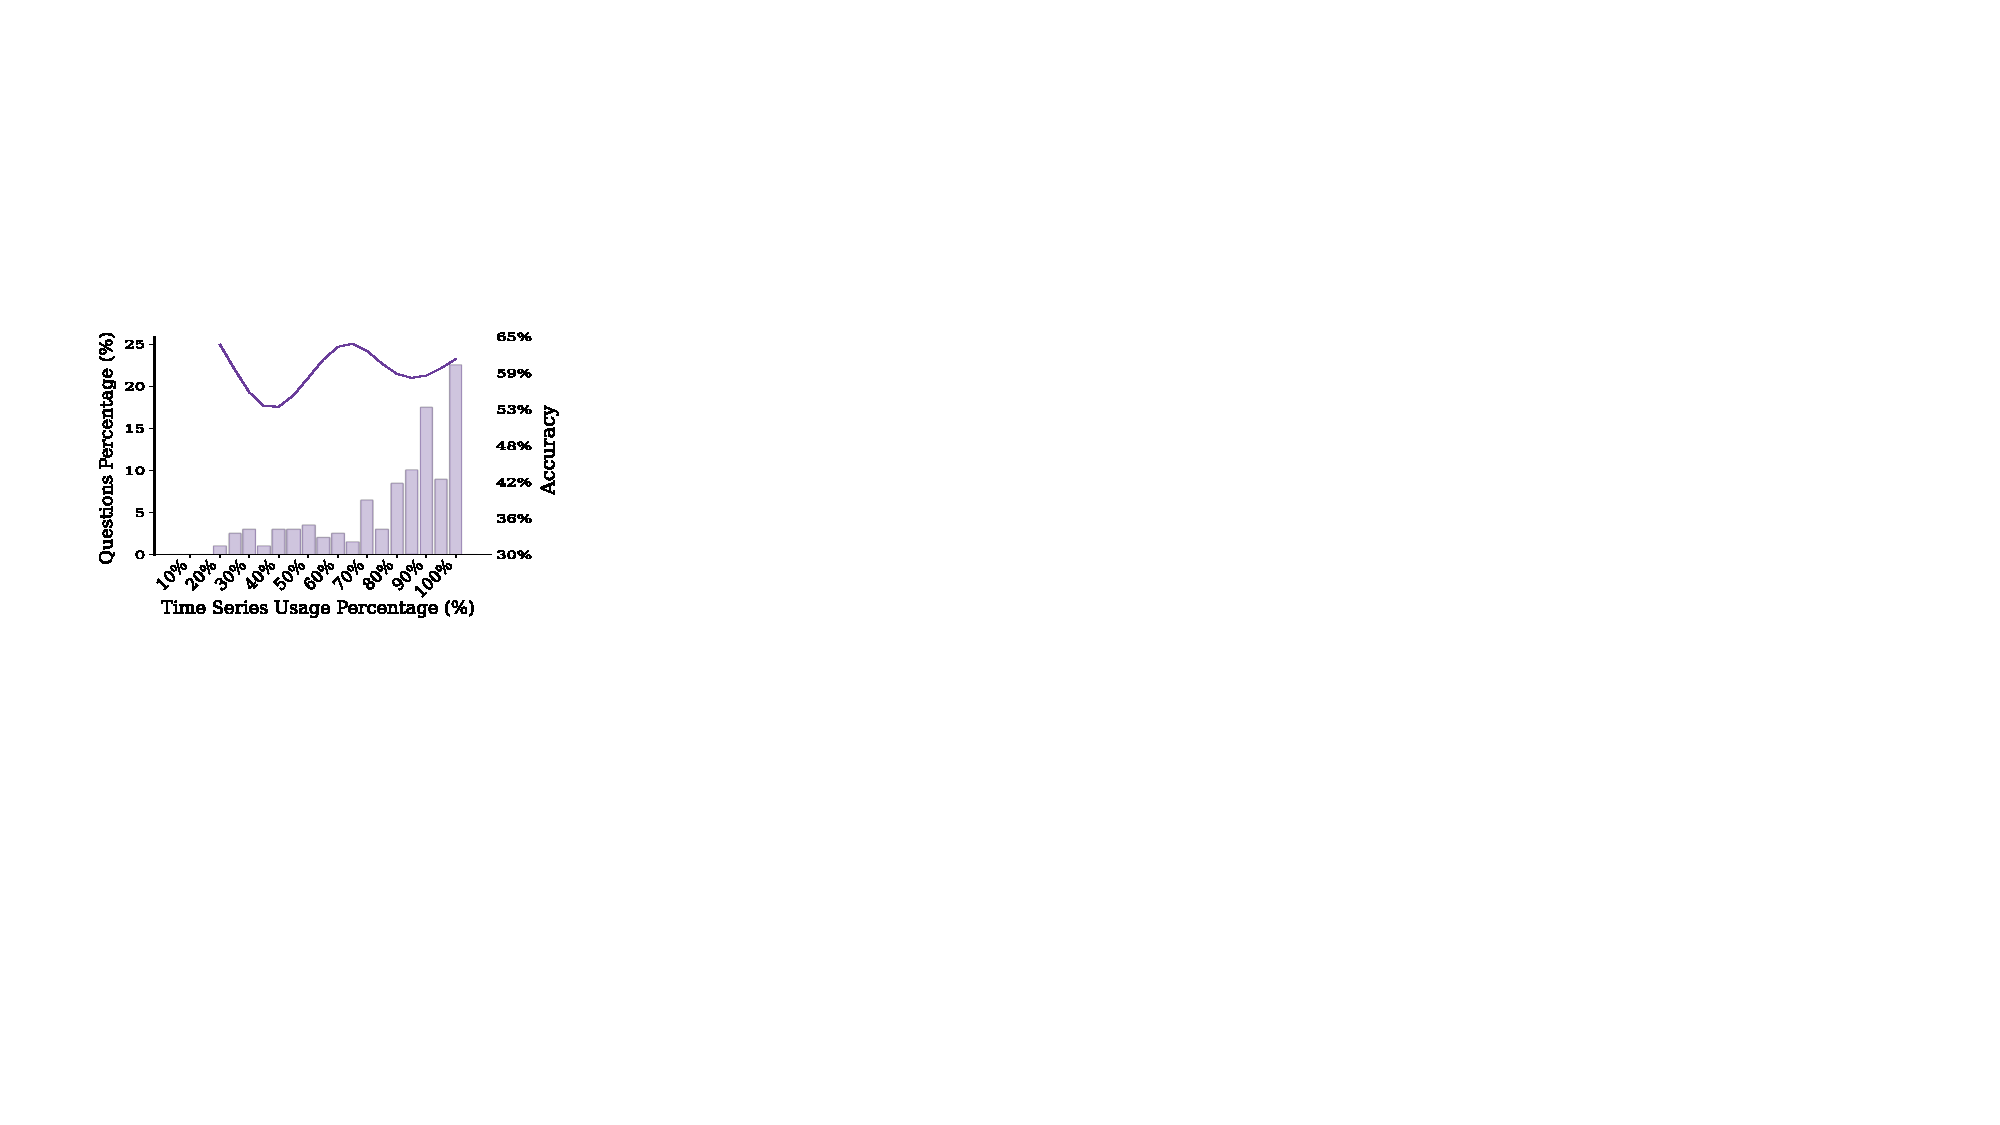
\includegraphics[width=\textwidth]{figs/usage_vs_acc_tsqa.pdf}
         \caption{TSQA.}
         \label{fig:usage_vs_acc_tsqa}
     \end{subfigure}
     \hfill
     \begin{subfigure}[b]{0.32\textwidth}
         \centering
         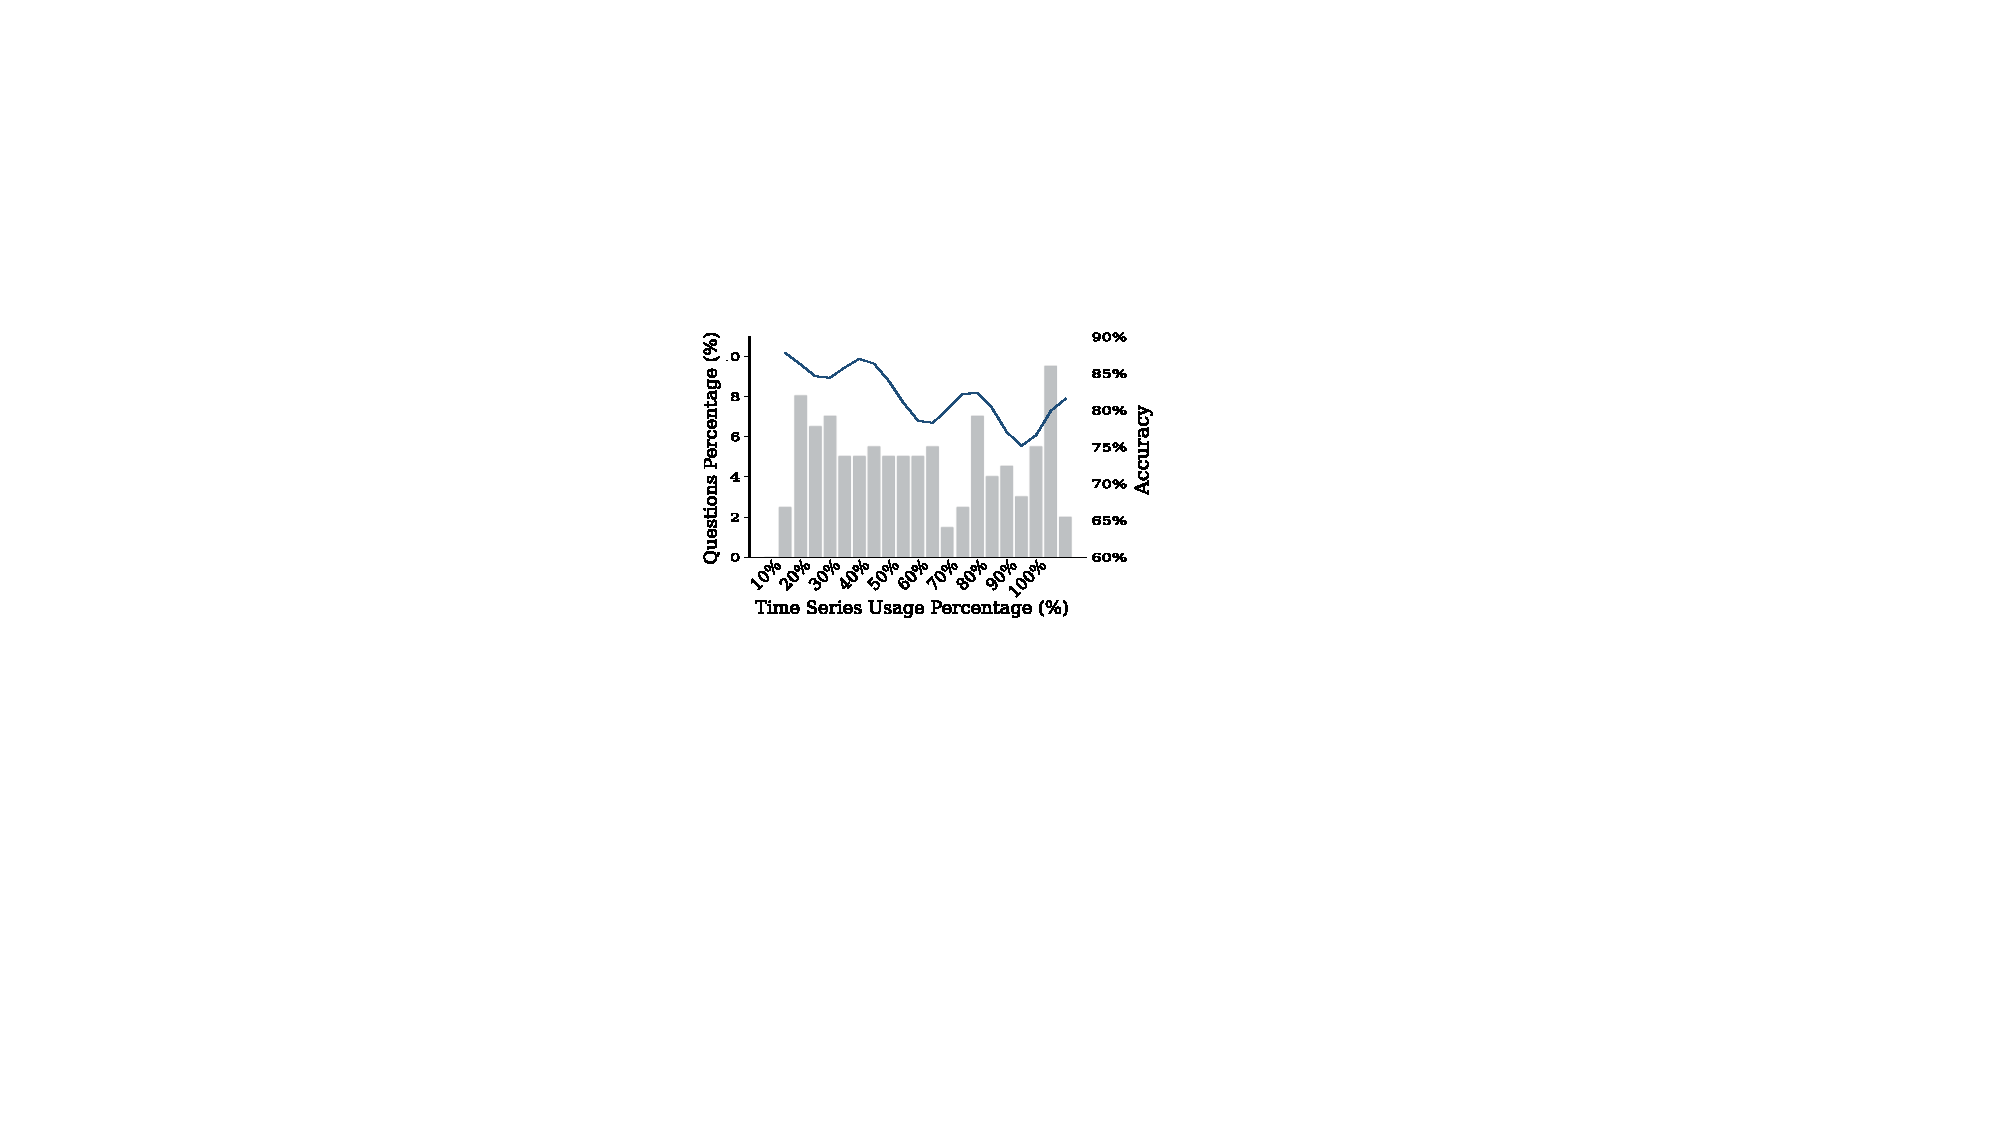
\includegraphics[width=\textwidth]{figs/usage_vs_acc_trqa.pdf}
         \caption{TRQA.}
         \label{fig:usage_vs_acc_trqa}
     \end{subfigure}
     \hfill
     \begin{subfigure}[b]{0.32\textwidth}
         \centering
         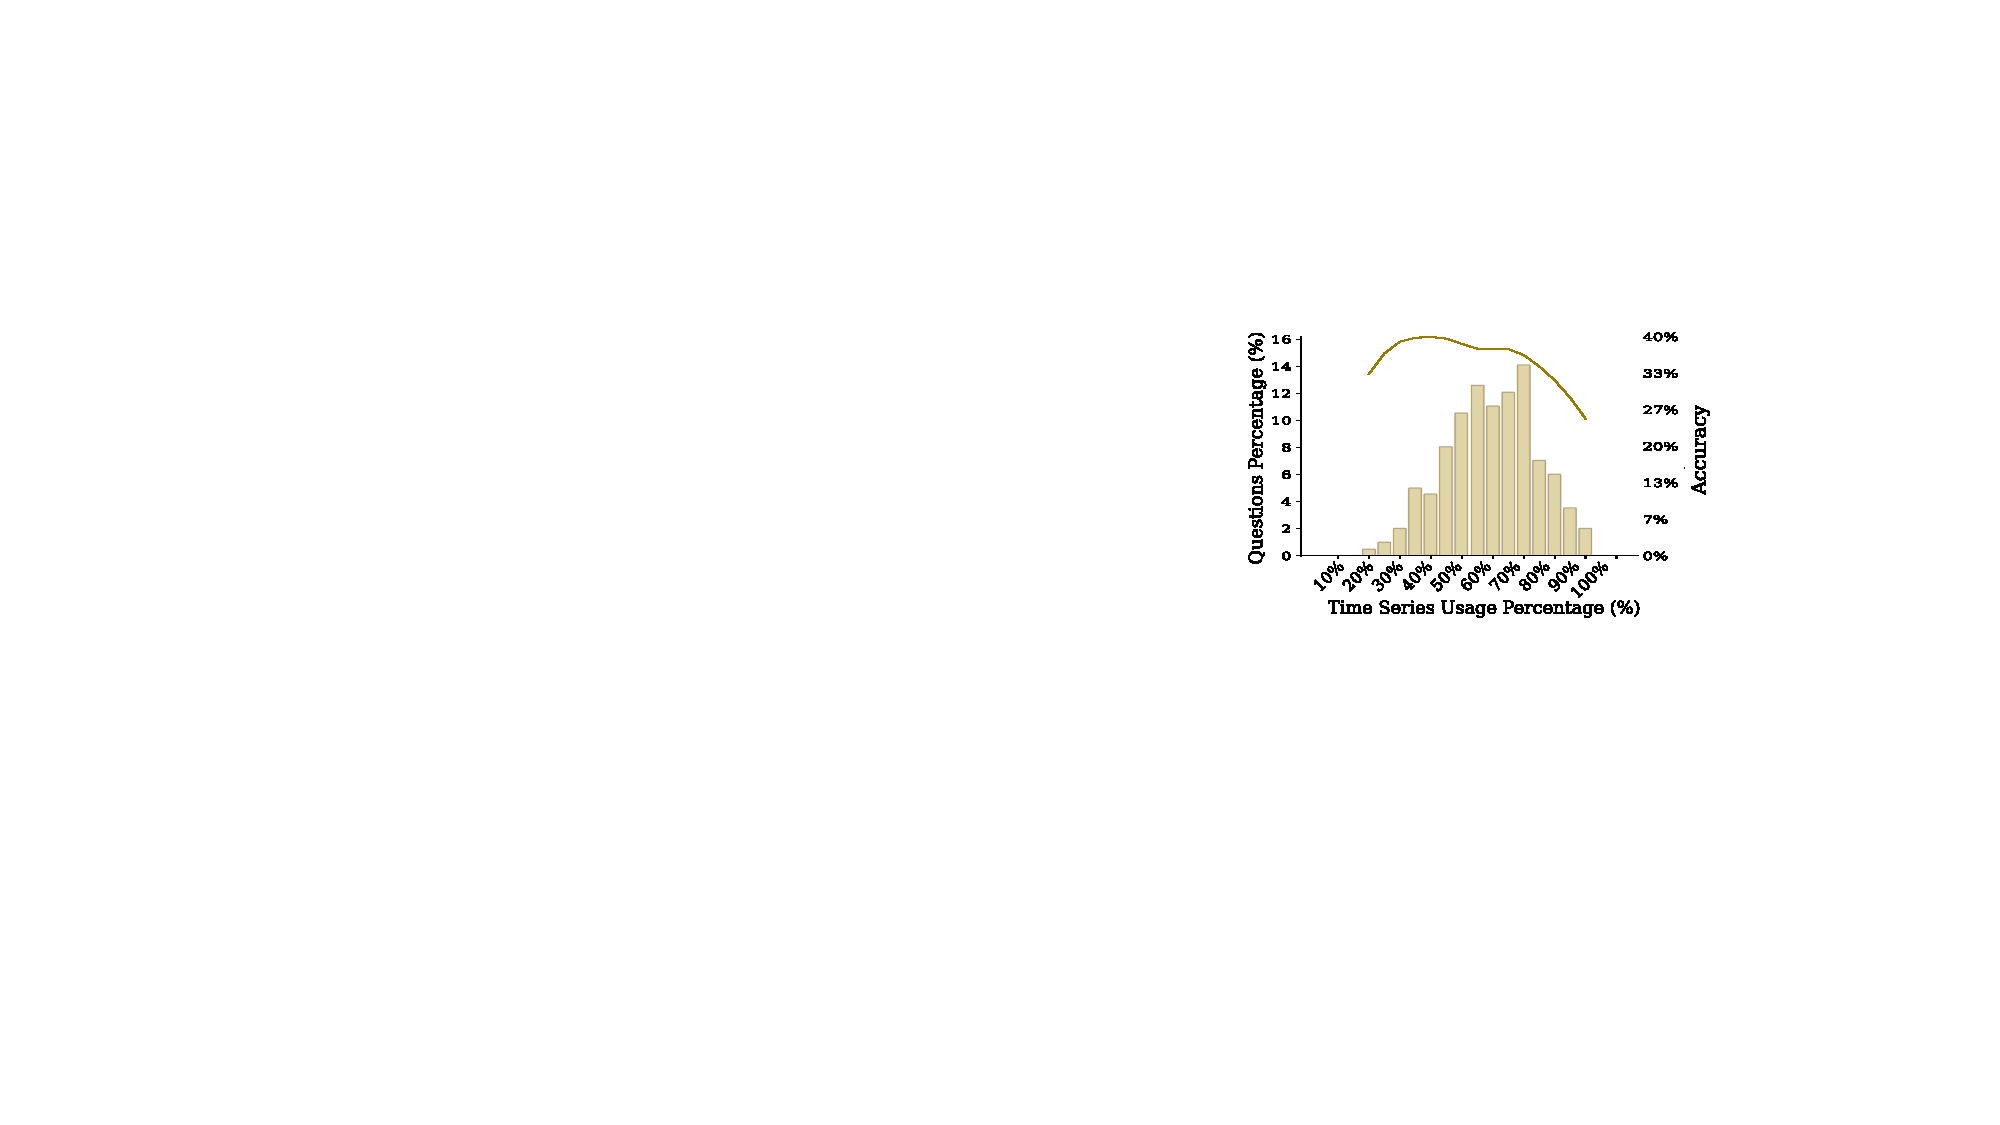
\includegraphics[width=\textwidth]{figs/usage_vs_acc_sleepqa.pdf}
         \caption{SLEEP QA.}
         \label{fig:usage_vs_acc_sleepqa}
     \end{subfigure}
     
     \caption{\textbf{Performance and question distribution across time-series usage levels.}
Bars (left axis) show the percentage of questions falling into each usage-percentage bin, and the line (right axis) shows accuracy for questions in that bin.}
     \label{fig:usage_vs_acc}
\end{figure*}

\textbf{Comparison with general LLMs and time-series reasoning models.}
Table~\ref{tab:multi_task_results} shows that ARTIST achieves the best overall performance across all benchmarks.
Relative to the strongest baseline on each dataset and metric, ARTIST improves average accuracy by 6.46\%.
RL further improves performance beyond SFT.
Compared with SFT, adding RL increases average accuracy from 63.61\% to 69.26\%.
\textbf{Comparison with vision--language reasoning models.}
Table~\ref{tab:image_based_baseline} compares ARTIST with VLM baselines that operate on plotted time series.
ARTIST is best on five of six datasets (ETI, RCW, ECG-QA, TSQA, TRQA), while TimeMaster+RL performs better on Sleep-QA.
We also observe that on ECG- and EEG-based datasets (ECG-QA and Sleep-QA), even VLMs without task-specific fine-tuning can be highly competitive, which may reflect stronger prior exposure to similar biomedical plots during pretraining.
To test whether this gap on Sleep-QA reflects a limitation of the segment selection mechanism or of the input modality itself, we additionally instantiate \algoname with a VLM backbone that consumes time series as plots. Under this representation, \algoname surpasses TimeMaster on Sleep-QA, indicating that the gap is primarily modality-driven rather than caused by the controller-reasoner design (Appendix~\ref{app:sleepqa_modality}).

\subsection{Analysis of Time Series Data Utilization}
Figure~\ref{fig:usage_vs_acc} examines how much of the time series \algoname uses under RL and how this relates to accuracy on three datasets.
Across datasets, greater coverage does not consistently improve performance.
Instead, accuracy is highest when the model concentrates on a limited set of question-relevant segments, and it drops for questions that trigger near-complete sequence usage.
For Sleep-QA and TRQA, the best accuracy occurs when the model uses roughly 30--50\% of the signal, whereas questions that induce 90--100\% utilization are substantially less accurate.
TSQA exhibits a higher optimal range (about 70\%), which is consistent with its shorter sequences and the need for proportionally broader coverage to capture relevant intervals.

\subsection{Ablation Study}
We conduct an ablation study to evaluate the core design choices of \algoname, with results summarized in Table~\ref{tab:ablation}.

\xhdr{Efficacy of Adaptive Segment Selection}
Removing the controller entirely, which processes the full time series as a static input, leads to a significant performance drop of 9.30\% in average accuracy. This confirms that processing the entire sequence can be suboptimal, as irrelevant temporal noise may obscure salient evidence. In contrast, ARTIST’s adaptive selection directs attention to task-relevant regions, enabling more precise reasoning.

\xhdr{Joint Controller-Reasoner Optimization}
\emph{Controller-only RL} configuration, where the reasoner remains frozen, results in an 8.94\% decrease in average accuracy compared to the full model. This degradation arises from a distribution shift: during RL, the reasoner is conditioned on a dynamically selected set of segments chosen by the controller, whereas in SFT it was trained under a different input regime, receiving the full time series followed by a small number of additional segments. Freezing the reasoner therefore prevents it from adapting to the controller’s evolving selection policy. Jointly updating both roles mitigates this mismatch and maintains alignment between segment selection and downstream reasoning.

\xhdr{Reliability Reward}
The most substantial performance decline (21.44\% average drop) occurs when removing the \emph{Reliability Reward}. Relying on single-rollout accuracy is insufficient due to the inherent stochasticity of LLMs: a reasoner may produce a correct answer by chance even when the selected segments are incomplete or irrelevant. In these cases, a single successful rollout can mislead the controller during learning. Our reliability metric uses nested rollouts to measure answer consistency across repeated samples. This estimate reflects whether the selected segment set reliably supports correct reasoning, rather than producing an isolated correct outcome.

\xhdr{Hierarchical Policy Optimization and Variance-Guided Sampling}
Replacing the trajectory-level objective with a myopic objective leads to a 12.28\% performance drop.
Here, the myopic objective refers to optimizing the controller based solely on the last interaction step, without propagating credit across the full interaction trajectory. With such an objective, the controller is encouraged to learn a greedy policy that is not optimized to make intermediate segment selections that lead to the best overarching segment set after multiple interactions.
%This prevents the controller from learning how intermediate segment selections contribute to long-term answer reliability. 
In contrast, our hierarchical objective trains the controller to optimize a sequence of segment selections that, together, forms an informative segment set.
%
Replacing \emph{Variance-guided Sampling} with standard stochastic sampling reduces average performance by 2.97\%.


\begin{table}[!t]
\centering
\caption{\textbf{Accuracy (\%) comparisons with vision  models.} }
\label{tab:image_based_baseline}
\small
\setlength{\tabcolsep}{2pt}
\resizebox{0.48\textwidth}{!}{
\begin{tabular}{lcccccc}
\toprule
\textbf{Model} &
\multicolumn{1}{c}{\textbf{ETI}} &
\multicolumn{1}{c}{\textbf{RCW}} &
\multicolumn{1}{c}{\textbf{ECG QA}} &
\multicolumn{1}{c}{\textbf{SLEEP QA}} &
\multicolumn{1}{c}{\textbf{TSQA}} &
\multicolumn{1}{c}{\textbf{TRQA}} \\
\midrule

Base Model
& 27.00 & 50.33 & 53.54 & 49.44 & 52.51 & 66.09 \\
VL-Time
& 28.50 & 57.52 & 58.91 & 22.06 & 44.93 & 53.50 \\
\quad  + Few-shot
& 22.00 & 48.67 & 64.36 & 23.53 & 38.16 & 58.50 \\

TimeMaster
& 26.00 & 67.70 & 52.59 & 47.51 & 58.30 & 68.45 \\
\quad + RL
& 49.00 & 76.99 & 69.31 & \textbf{72.55} & 61.22 & 72.08 \\

\midrule

\algoname & & & & & & \\
\rowcolor{lightpurple}
% \quad + SFT \\
\quad + SFT & 85.12 & 69.75 & 56.31 & 28.13 & 60.06 & 82.26 \\
\rowcolor{lightpurple}
% \quad + RL + SFT \\
\quad + RL + SFT & \textbf{87.03} & \textbf{77.00} & \textbf{69.81} & 36.63 & \textbf{62.00} & \textbf{83.34} \\
\bottomrule
\end{tabular}
}
\vspace{-3mm}
\end{table}

\begin{figure*}[]
     \centering
     \begin{subfigure}[b]{0.48\textwidth}
         \centering
         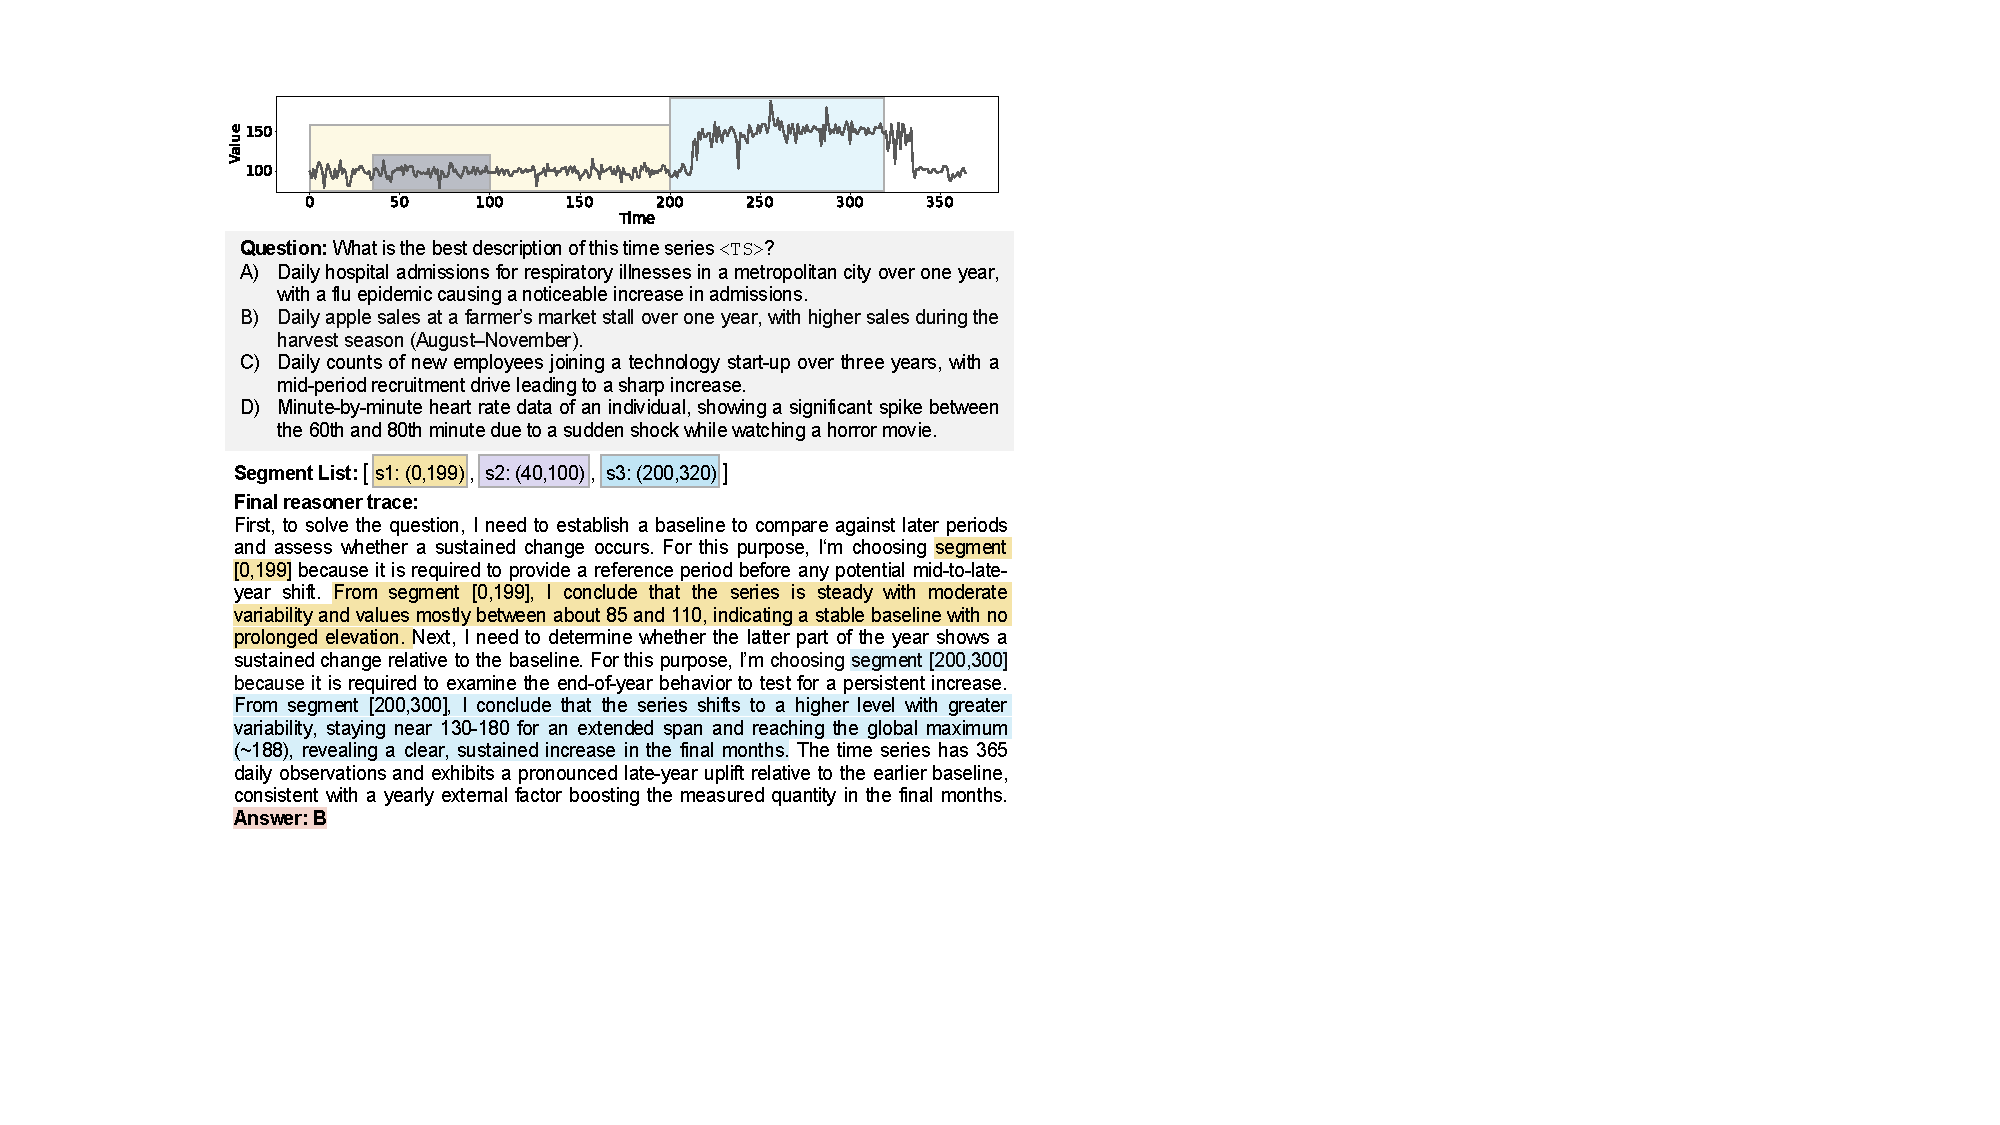
\includegraphics[width=\textwidth]{figs/case_study1.pdf}
         % \caption{Apple sales data.}
         \label{fig:case_retail}
     \end{subfigure}
     \hfill 
     \begin{subfigure}[b]{0.48\textwidth}
         \centering
         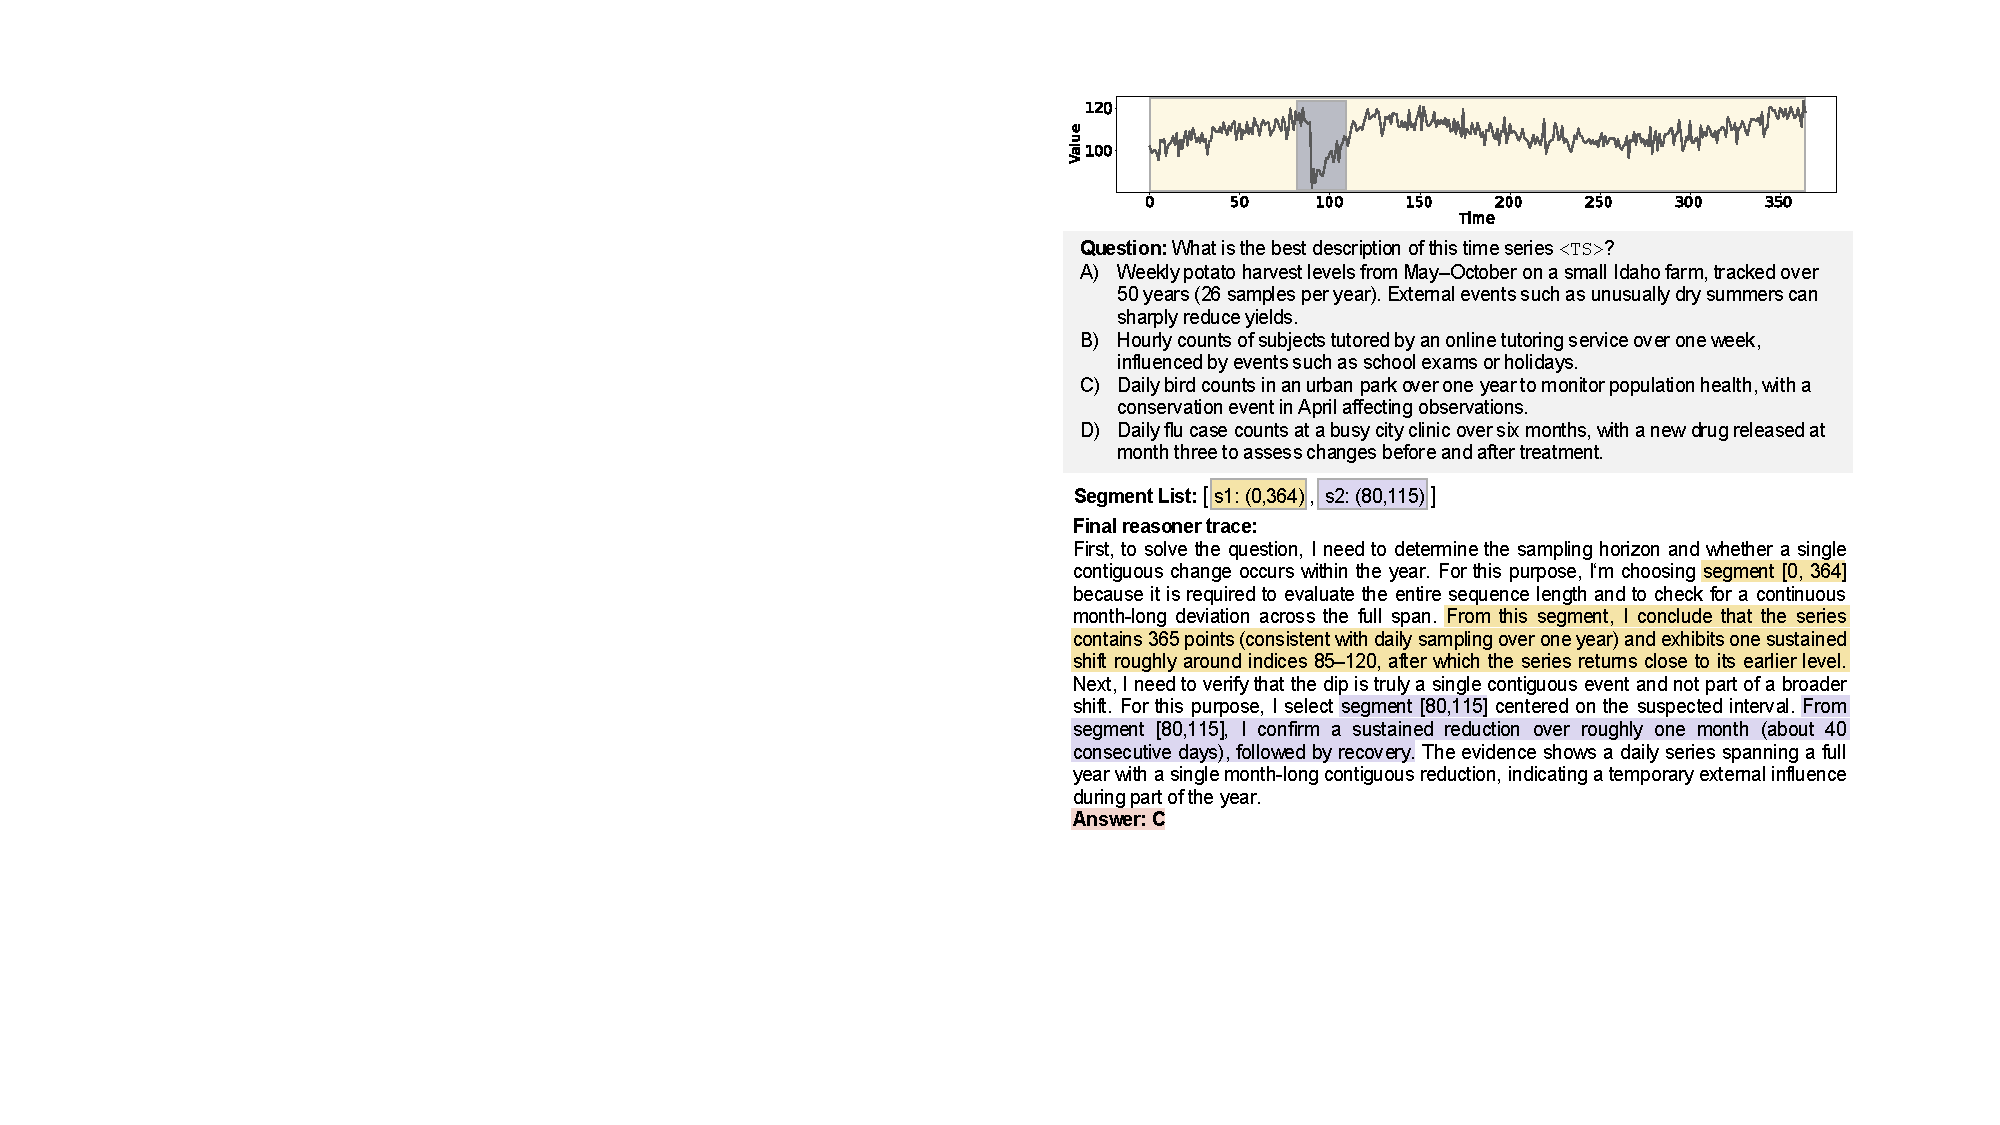
\includegraphics[width=\textwidth]{figs/case_study2.pdf}
         % \caption{Bird count monitoring.}
         \label{fig:case_ecology}
     \end{subfigure} 
     \vspace{-4mm}
     \caption{\textbf{Examples of using \algoname for reasoning with time series.} Source: Etiological time series reasoning bechmark.}
     \label{fig:total_figure}
\end{figure*}

\begin{table}[t]
\centering
\small
\caption{\textbf{Ablation on ECG-QA and RCW accuracy (\%).}}
\label{tab:ablation}
\setlength{\tabcolsep}{5pt}
\begin{tabular}{lccc}
\toprule
\textbf{Method} & \textbf{ECG} & \textbf{RCW} & \textbf{Avg.} \\
\midrule
\rowcolor{lightpurple}
\algoname & \textbf{69.81} & \textbf{77.00} & \textbf{73.41} \\
Reasoner Only & 65.33 & 62.88 & 64.11 \\
Controller-only RL & 60.81 & 68.13 & 64.47 \\
\midrule
w/o Reliability Reward & 52.50 & 51.44 & 51.97 \\
w/o Trajectory-based Objective & 55.19 & 67.06 & 61.13 \\
w/o Variance-guided Sampling & 68.13 & 72.75 & 70.44 \\
\bottomrule
\end{tabular}
\vspace{-3mm}
\end{table}




\subsection{Illustration of Time Series Reasoning in \algoname}
Figure~\ref{fig:total_figure} illustrates how \algoname addresses queries by selecting a targeted set of informative segments. 
In the apple sales case (Figure~\ref{fig:total_figure},left), the controller first retrieves an early segment to establish a baseline level. Guided by the initial hypothesis of a potential trend shift, it then queries a late-sequence segment to test whether the change persists. The retrieved segment reveals a sustained level increase with higher variability, allowing the model to confirm a seasonal harvest uplift rather than a transient spike. 
In the bird count example (Figure~\ref{fig:total_figure},right), the model begins with a full-span segment to establish the sampling horizon and flag suspicious intervals. It then requests a higher-resolution segment around the anomaly to determine its duration and whether the signal recovers. This second segment shows a contiguous dip on the scale of months followed by a return to the prior level, which supports a temporary external influence rather than a persistent regime change.
%
Segment selection yields a verifiable evidence trail that ties the final answer to specific temporal segments. 